\documentclass[10pt, aspectratio=169]{beamer}
\usepackage{udec-slides}
\slide{7}{Ley de Biot-Savart}

\begin{document}
\primeraDiapo

\begin{frame}{Ley de Biot-Savart}
    La ley de Biot-Savart describe cómo una corriente eléctrica constante genera un campo magnético $\vec{B}$ en un punto del espacio.

    \begin{boxTeoria}{Definición Diferencial}
        El campo magnético infinitesimal $d\vec{B}$ producido por un elemento de corriente $I d\vec{l}$ a una distancia $r$ se expresa como:
        \begin{equation*}
            d\vec{B} = \frac{\mu_0}{4\pi} \frac{I d\vec{l} \times \hat{r}}{r^2} \quad [\unit{\tesla}]
        \end{equation*}
    \end{boxTeoria}

    \begin{itemize}
        \item \textbf{Geometría:} El vector $d\vec{B}$ es perpendicular tanto al elemento de corriente $d\vec{l}$ como al vector unitario radial $\hat{r}$ (regla de la mano derecha).
        \item \textbf{Constante ($\mu_0$):} Representa la permeabilidad magnética del vacío, cuyo valor exacto es $4\pi \times 10^{-7} \, \unit{\tesla\cdot\meter/\ampere}$.
    \end{itemize}
\end{frame}

\begin{frame}{Problema 1}{Segmento de corriente finito}
    Deducir una expresión general para el campo magnético $\vec{B}$ en un punto $P$ a una distancia perpendicular $h$ de un conductor recto que se extiende desde $x=a$ hasta $x=b$ sobre el eje $x$. Esta fórmula fundamental servirá como base para resolver aplicaciones futuras.

    \begin{figure}[h]
        \centering
        \resizebox{0.5\textwidth}{!}{%
            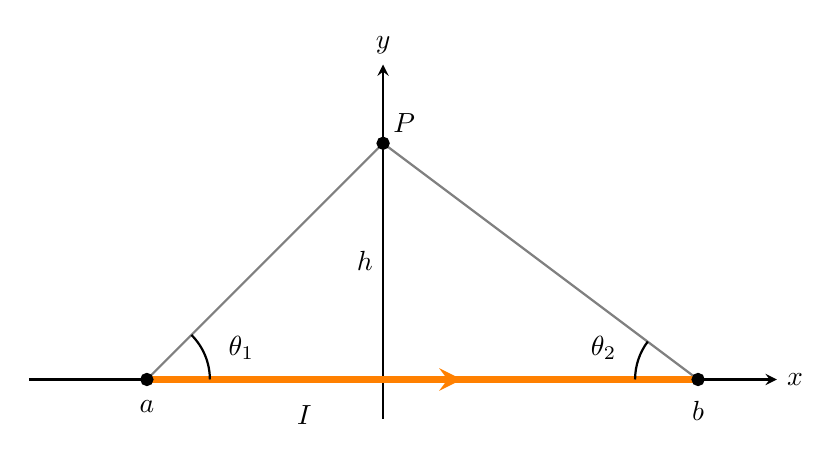
\begin{tikzpicture}[>=stealth, thick]
                % Ejes de coordenadas
                \draw[->] (-4.5,0) -- (5,0) node[right] {$x$};
                \draw[->] (0,-0.5) -- (0,4) node[above] {$y$};

                % Rayos de proyección hacia el punto P desde los extremos (Líneas continuas)
                \draw[black!50, line width=0.8pt] (-3,0) -- (0,3);
                \draw[black!50, line width=0.8pt] (4,0) -- (0,3);

                % Conductor sobre el eje x (desde a hasta b)
                \draw[orange, line width=2.5pt] (-3,0) -- (4,0);

                % Etiqueta de la Corriente e indicación de sentido
                \draw[->, orange, line width=2.5pt] (-3,0) -- (1,0) node[midway, below=5pt, black] {$I$};

                % Puntos de los extremos
                \filldraw (-3,0) circle (2pt) node[below=4pt] {$a$};
                \filldraw (4,0) circle (2pt) node[below=4pt] {$b$};

                % Punto P de interés y etiqueta de altura h
                \filldraw (0,3) circle (2pt) node[above right] {$P$};
                \node[left] at (0,1.5) {$h$};

                % Ángulo theta_1 en el extremo 'a'
                % El arco cierra perfectamente con el rayo hacia P (45 grados)
                \draw[thick] (-2.2,0) arc (0:45:0.8);
                \node at (-1.8, 0.4) {$\theta_1$};

                % Ángulo theta_2 en el extremo 'b'
                % El arco cierra perfectamente con el rayo hacia P (143 grados internos)
                \draw[thick] (3.2,0) arc (180:143:0.8);
                \node at (2.8, 0.4) {$\theta_2$};

            \end{tikzpicture}%
        }
    \end{figure}
\end{frame}

\begin{frame}{Problema 2}{Espira circular}
    Considerando un conductor con forma de espira circular de radio $R$ que lleva una corriente $I$:
    \begin{itemize}
        \item Determine el valor del campo magnético en el centro de la espira.
    \end{itemize}
    \begin{figure}
        \centering

        \resizebox{0.25\textwidth}{!}{%
            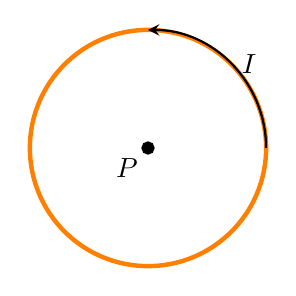
\begin{tikzpicture}[>=stealth, thick]
                % Espira
                \draw[orange, ultra thick] (0,0) circle (1.5cm);
                \draw[->] (1.5,0) arc (0:90:1.5) node[midway, right] {$I$};

                % Centro y campo
                \filldraw (0,0) circle (2pt) node[below left] {$P$};

            \end{tikzpicture}%
        }
    \end{figure}

\end{frame}

\begin{frame}{La Fuerza de Lorentz}
    Fuerza total sobre una carga $q$ que se mueve con velocidad $\vec{v}$ en presencia de campos $\vec{E}$ y $\vec{B}$.

    \begin{boxTeoria}{Expresión General}
        \begin{equation*}
            \vec{F} = q (\vec{E} + \vec{v} \times \vec{B})
        \end{equation*}
    \end{boxTeoria}

    \begin{itemize}
        \item \textbf{Fuerza Magnética ($\vec{F}_m$):} Si $\vec{E} = 0$, la fuerza es puramente magnética: $\vec{F}_m = q (\vec{v} \times \vec{B})$.
        \item \textbf{Geometría:} $\vec{F}_m$ siempre es \textbf{perpendicular} tanto a la velocidad $\vec{v}$ como al campo $\vec{B}$ (Regla de la mano derecha).
        \item \textbf{Efecto Físico:} Al ser perpendicular al desplazamiento, el campo magnético \textbf{no realiza trabajo}. Solo curva la trayectoria de la partícula sin alterar su rapidez.
    \end{itemize}
\end{frame}

\begin{frame}{Ejercicio: Campo Magnético y Dinámica de Partículas}
    Un alambre rectilíneo de cobre muy largo, de radio $1 \, \unit{\milli\meter}$, es recorrido por una corriente constante de $20 \, \unit{\ampere}$.

    Determine de manera vectorial:
    \begin{enumerate}[a)]
        \item La fuerza magnética instantánea que se ejerce sobre uno de los electrones de conducción que se desplaza a una velocidad de $10^{6} \, \unit{\meter/\second}$ a lo largo de la superficie del alambre, en sentido opuesto al de la corriente eléctrica.
        \item La aceleración correspondiente que experimenta dicho electrón producto de la interacción con el campo magnético del conductor.
    \end{enumerate}

    \vspace{0.3cm}
    \begin{small}
        \textbf{Datos útiles:}
        \begin{itemize}
            \item Carga del electrón: $e = -1.602 \times 10^{-19} \, \unit{\coulomb}$
            \item Masa del electrón: $m_e = 9.109 \times 10^{-31} \, \unit{\kilogram}$
            \item Permeabilidad del vacío: $\mu_0 = 4\pi \times 10^{-7} \, \unit{\tesla\cdot\meter/\ampere}$
        \end{itemize}
    \end{small}
\end{frame}


\end{document}